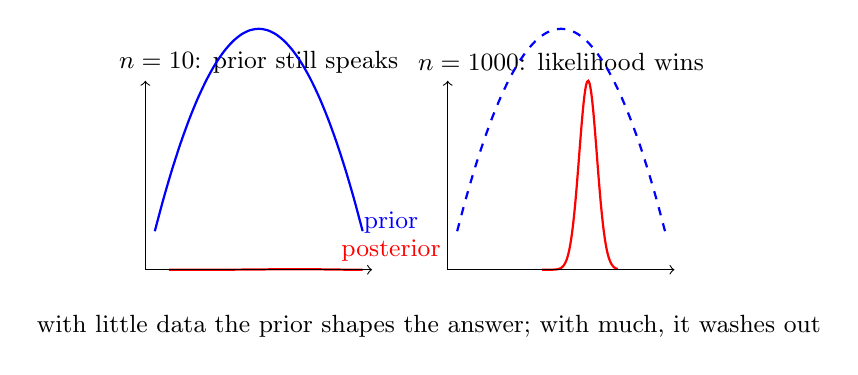
\begin{tikzpicture}[scale=0.6]
\begin{scope}
\node at (2.4,4.4) {\small $n=10$: prior still speaks};
\draw[domain=0.2:4.6,smooth,thick,blue] plot (\x,{3.4*(\x/4.8)*(1-\x/4.8)*6});
\draw[domain=0.5:4.6,smooth,thick,red,samples=50] plot (\x,{24*((\x/4.8)^8*(1-\x/4.8)^4)});
\draw[->] (0,0)--(4.8,0); \draw[->] (0,0)--(0,4);
\end{scope}
\begin{scope}[xshift=6.4cm]
\node at (2.4,4.4) {\small $n=1000$: likelihood wins};
\draw[domain=0.2:4.6,smooth,thick,blue,dashed] plot (\x,{3.4*(\x/4.8)*(1-\x/4.8)*6});
\draw[domain=2.0:3.6,smooth,thick,red,samples=60] plot (\x,{4.0*exp(-((\x-2.97)^2)/0.07)});
\draw[->] (0,0)--(4.8,0); \draw[->] (0,0)--(0,4);
\end{scope}
\node[blue] at (5.2,1.0) {\small prior};
\node[red] at (5.2,0.4) {\small posterior};
\node at (6.0,-1.2) {\small with little data the prior shapes the answer; with much, it washes out};
\end{tikzpicture}
